\section{Experimental Results}\label{section:experiments-results}

\subsection{Quantitative Results}\label{subsec:quantitative}

As discussed in the previous session, the four NEAT variants were
compared in two ways: First we perform three full evolution runs for
each variant/matchup pairing, and then the five best genomes obtained
from this training are run 50 times to evaluate their victory and
survival ratios. A summary of these results is presented in
Table~\ref{table:quantitative}.

\begin{table}
    \caption{Victory Ratio and Median Survival for the best genomes.
            Survival values only consider victory matches.}
    \label{table:quantitative}
    \begin{tabular}{llll}
        \toprule
        Variant & Matchup & Win Ratio & Survival \\
        \midrule
        Vanilla & marine/marine & 0.77 & 8 \\
        Unified & marine/marine & 0.77 & 8 \\
        Cascade & marine/marine & 0.85 & 8 \\
        Novelty & marine/marine & 0.55 & 8 \\[1ex]

        Vanilla & marine/zergling & 0.03 & 4 \\
        Unified & marine/zergling & 0.01 & 10 \\
        Cascade & marine/zergling & 0.05 & 5 \\
        Novelty & marine/zergling & 0.09 & 10 \\[1ex]

        Vanilla & vulture/vulture & 0.92 & 8 \\
        Unified & vulture/vulture & 0.90 & 10 \\
        Cascade & vulture/vulture & 0.93 & 8 \\
        Novelty & vulture/vulture & 0.93 & 9 \\[1ex]

        Vanilla & vulture/zealot & 0.87 & 8 \\
        Unified & vulture/zealot & 0.93 & 9 \\
        Cascade & vulture/zealot & 0.92 & 9 \\
        Novelty & vulture/zealot & 0.99 & 9 \\
        \bottomrule
    \end{tabular}
\end{table}

% \subsubsection{Victory Rate Analysis}

From this table, we can observe that in general the methods managed to
learn a good tactic to defeat their enemies, with the exception of the
marine/zergling matchup.
%\footnote{This could be considered scientific evidence that Blizzard needs to nerf zerglings}
Small variations are observed on the methods within each matchup, but
an ANOVA test confirms that these variations are not significative (F
= 0.85).

% \subsubsection{Survival Rate Analysis}

In the same fashion, it was not possible to observe a clear difference
among the variants in terms of the median number of survivors in
winning matches. Figure~\ref{fig:survivors} shows the survivor numbers
for each variation/matching pairing.

\begin{figure}
  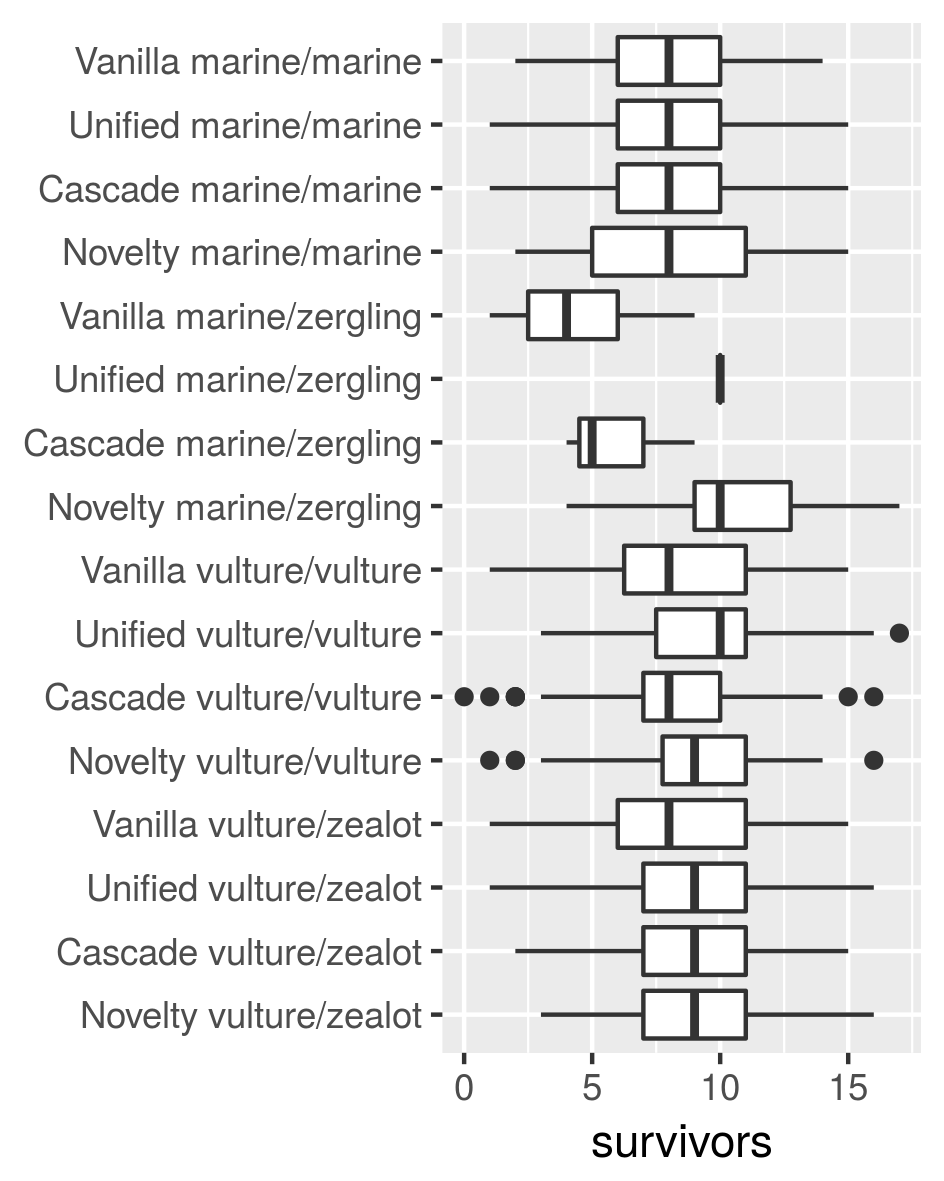
\includegraphics[width=.5\textwidth]{figures/survivors}
  \caption{Box plot for the survival ratios}\label{fig:survivors}
\end{figure}

% \subsubsection{Evolution Rate Analysis}


\begin{figure*}
  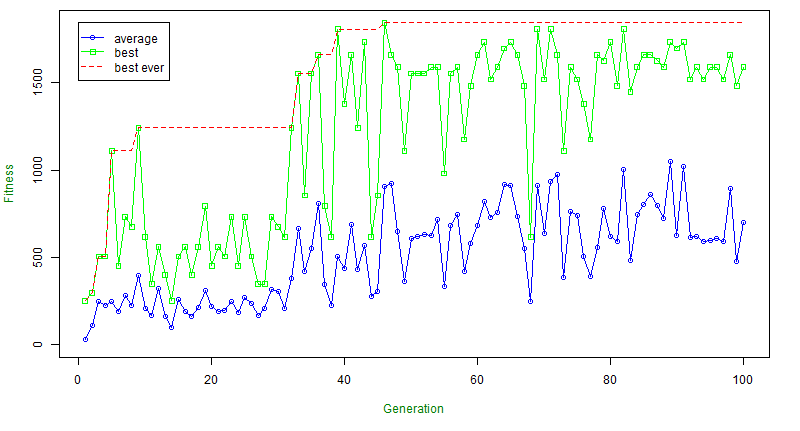
\includegraphics[width=.4\textwidth]{figures/evolution_zealot}
  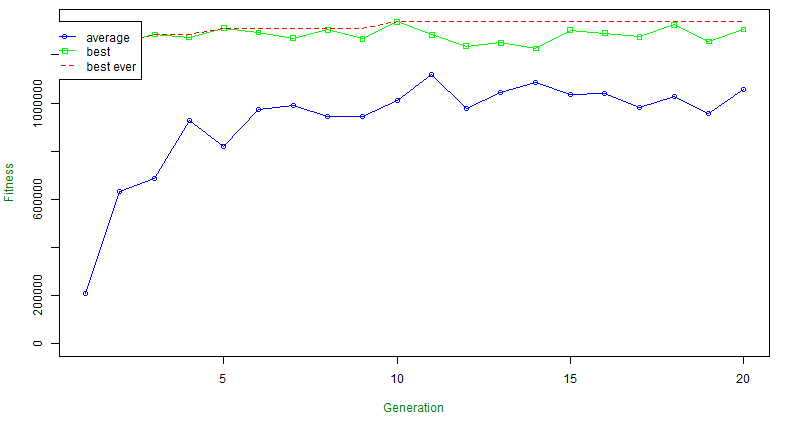
\includegraphics[width=.4\textwidth]{figures/evolution_unified}
  \caption{Training progress for two vulture vs zealot matchups. Left:
    Cascade NEAT vs zealots. Right: Unified NEAT. Note that the
    fitness function are different so absolute values should not be
    compared directly.}\label{fig:evolution}
\end{figure*}

Finally, we observed the training progress of the
experiment. Figure~\ref{fig:evolution} show two examples of training
graphs that are representative of the experiment as a
whole\footnote{the figures for all matchings can be found at the
online repository}. In the Cascade NEAT training (left side) we see
that while there is a small increase in best and mean fitness, there
are large variations every generation. In the Unified NEAT training
(right side) these variations are not present. In unified neat, all
networks in the same combat experiment share the same fitness result,
while in the other variants (such as the Cascade Neat) each network in
the same combat is evaluated separately, even though they influence
each other (a weak network will make the overall combat harder for a
stronger network).

However, while this difference is observable in the training curve, as
we see in Figure~\ref{fig:evolution}, it did not generate an
observable difference in the final result
(Table~\ref{table:quantitative}), which is interesting.

\subsection{Qualitative analysis}\label{subsec:qualitative}

From the quantitative analysis we learned that a winning strategy was
generally found (high winning ratio), while the differences among
variants was not strong. In particular, the survivor rate was the same
across methods with the exception of the particularly hard
marine/zergling matchup.

To better understand this lack of difference, and what could be done
to increase the survival ratio, we performed a qualitative analysis of the
results of the experiment by studying the different behaviors that emerged.

\subsubsection{Developping stimpack behaviour}

\begin{figure}
    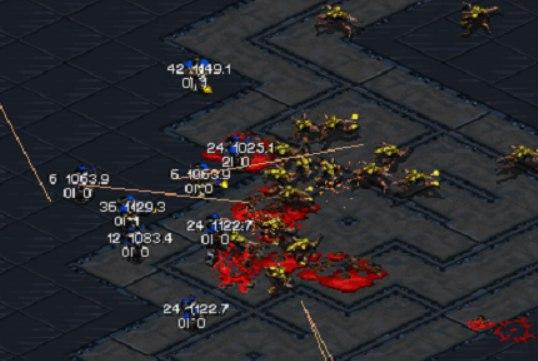
\includegraphics[width=.45\textwidth]{figures/marines_vs_zerglings_combat}
    \caption{Marines/Zerglings Matchup. The Zergling speed makes this
      a hard matchup to win without stimpack
      behavior}\label{fig:marines_vs_zerglings}
\end{figure}

The Marine/Zergling matchup was the hardest one of the four studied,
and the one where none of the NEAT variants managed to consistently
find a good solution. This is because the high speed of the zerglings
prevent the marines from develop a kiting behavior
(Figure~\ref{fig:marines_vs_zerglings}).

To solve this problem, an agent needs to develop a \emph{stimpack
  behavior}. Stimpack is an ability that increases the speed of the
marine for a few seconds, in exchange of an amount of its health. 

Vanilla NEAT and Cascade NEAT didn't do a good job at developing this
stimpack behavior. What we observed is that in a population where some
individuals use stimpack and some don't, the individuals that do not
use stimpack get better reward (because of their health), even though
their survival is because of the 'sacrifice' of the stimpack using
individuals, who rushed to the frontline and got themselves killed
first. The final result is that the stimpack behavior gets lost over
the generations.

In comparison, the Unified Variant was somewhat better at developing
the stimpack behavior. Since all agents in one combat use the same
genotype and have the same genotype, all of them are rewarded equally
for the use of stimpack, even if some units are lost early.

As for the Novelty Variant, the behavior is lost less easily, and some
of the best genomes still use it. However, there is still a degree
of loss during the evolution, specially when some units in combat develop
a fleeing behavior. However, the novelty aspect might be just enough to
keep the less rewarded stimpack users in the gene pool, and help explain the
better result of novelty search noticed in the previous section.

Overall, another reason for losing the stimpack behavior is the timing
of its development during the training. If the fighting behavior is
poor (for instance, not attacking the enemy or fleeing without
reason), stimpack usage will exarcebate the problem. We imagine that
it might be possible to develop a good stimpack behavior with a better
novelty measurement that does not use the fitness and more
appropriately model the novelty of combat behaviors.

Additionaly, the marines vs marines matchup is solved differently from
the zergling matchup. We observed that in most cases this matchup can
be won by just waiting for the enemy and attacking all at once without
stimpack, which was precisely the convergent behavior. This happens
because the initial enemy formation may lead to a line to form during
their advance, meaning that if the squad holds its original position
it can pick the enemy forces a part at a time, shooting first with
more firepower.

\subsubsection{Kiting behaviour}

\begin{figure}
    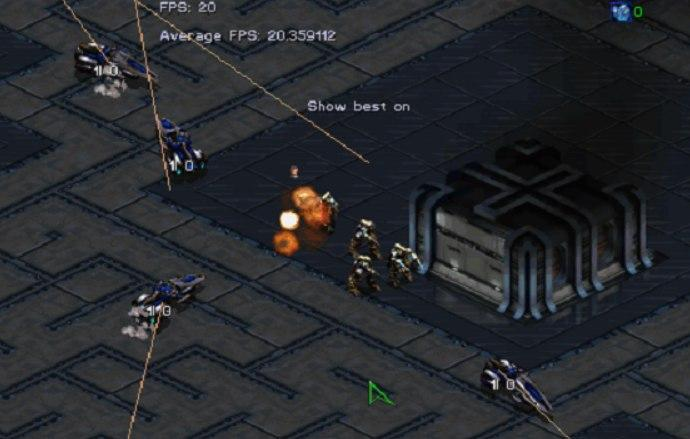
\includegraphics[width=.45\textwidth]{figures/vultures_kiting_screenshot}
    \caption{Vultures using kiting technique to beat
      zealots}\label{fig:vultures_kiting}
\end{figure}

All the studied variants performed exceedingly well on the
vulture/zealot matchup, as described in
section~\ref{subsec:quantitative}. This matchup illustrates the
\emph{kiting behavior}, where a faster, long ranged unit has to keep a
distance from a short ranged opponent.


After a short number of generations, adequate individuals start to
emerge, even with the first species, meaning the topology required
isn’t complex at all. After a few more generations, networks weights
are tweaked to get a quite decent kiting behaviour for any variant.
The vulture is able to maintain a good distance between itself and the
enemies as shown on Figure~\ref{fig:vultures_kiting}. In some cases,
vultures are even able to shoot without losing speed and thus withdraw
really quickly from risks. This ressemble a classical vulture micro
technique called “patrol micro” involving the use of the so-called
patrol command's lack of cooldown to have the vulture move, fire, and
retreat without slowing down. We don’t really know how it is achieved
here without the patrol command, but it is effectively the same
result.

It is interesting to note that for the matchup vultures vs vultures,
our bot was even more effective by avoiding opponent's projectiles
using, again, effective kiting. Although the vulture projectiles do
not instantly hit their targed as the marine's do, it was impressive
that they could shine against an identical opponent.

\subsubsection{Spread out behaviour}\label{subsec:spreading}

\begin{figure}
    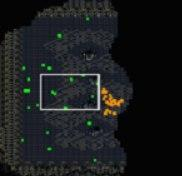
\includegraphics[width=.22\textwidth]{figures/spreading_behaviour_standard_neat}
    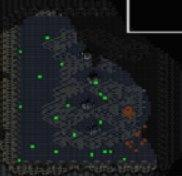
\includegraphics[width=.22\textwidth]{figures/spreading_behaviour_unified}
    \caption{Spread out behaviour with standard NEAT (left) and Unified Variant (right)}\label{fig:spreading-behaviour}
\end{figure}

In the vulture match ups, another interesting behaviour was the
vultures spreading out to cover a large area (see
Figure~\ref{fig:spreading-behaviour}) and then converge back to the
enemy once it's spotted.

However, this behaviour tends to disappear like the stimpack behavior,
probably because the fitness of these individuals is not as good for
various reasons.  It may be because spreading out and converging back
takes time and lead to less damages inflicted or because some
individuals which had the spreading behaviour without attacking
afterward, especially for the Unified Variant where the behaviour is
often lost very quickly when not even a single unit tries to attack.
Moreover, we didn't see the behaviour at all with Cascade-NEAT, but it
may be due to randomness.

\begin{figure}
    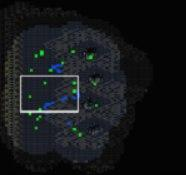
\includegraphics[width=.25\textwidth]{figures/spreading_behaviour_novelty}
    \caption{Spread out behaviour with the Novelty Variant}\label{fig:spreading-behaviour-novelty}
\end{figure}

That being said, novelty search found a very efficient spreading
behaviour leading to a complete encirclement of the oponent as show in
Figure~\ref{fig:spreading-behaviour-novelty}.

